\section{CLI app improvements}\label{sec:cli-app-improvements}
Our CLI app is based on~\nameref{subsec:git-time-metric}, an already working open source time tracking app.
Although it already had all the basic features, some improvements and fixes were required.

Firstly \textit{--cwd=\{some/path\}} option was added to allow easier integration of plugins.
Option to pass current directory as option is required, as IDEs not launched from terminal sometimes have their working
directory elsewhere and setting custom working directory every time we call CLI app is more complicated than passing an argument.

To clean up user home directories, global config files were moved from \textit{~/.git-time-metrics/} to \textit{~/.config/gtm/}.
For windows a new installer was built to make installing easier.
Also, it was chosen to switch from statically compiling SSH2 Libraries into our application to dynamic linking.
For Debian Linux, a build script for debian packages was set up to also provide debian packages with every release.

The application was updated to automatically add a fetch refspecs to fetch data from remotes on git fetch.
Also, a pre-push git hook was added to automatically push data to origin.
With these two hooks, the time data is automatically fetched pushed whenever git push is made requiring user no extra effort.

To still allow users to only track time locally, a \textit{--local} option was added to \textit{init} command.
Also \textit{--auto-log=[jira|gitlab]} option was added to support automatic time logging to commit messages.
Currently, this time can only be collected in Jira, but there is also and \href{https://gitlab.com/gitlab-org/gitlab/-/issues/16543}{issue}
open for Gitlab to implement this.

To view data based branch the checked out branch name when the commit was made is also now stored to data.
This couldn't be avoided because the branch is simply a pointer to commit and due to git being distributed control system,
it isn't guaranteed.

For students, it is important to view time spent on specific tasks.
In most subjects the tasks are placed in separate subdirectories for better files management.
To allow users to view time spent on specific tasks, a \textit{--subdir="sub/dir/name"} option was added to filter out
data based on directories.

Although the Git supports automatic merging/rewriting of the notes, it was inconsistent in some cases, especially when the user
wants to also rewrite manually added notes.
To keep time data after Git rebases, a new command \textit{rewrite} was introduced.
This command is ran by git post-rewrite hook, and it rewrites notes so that they still point to correct commit.

\section{Groups system}\label{sec:group-system}
One of the requirements for our app was that it should be possible to group repositories together.
The grouping is needed to view statistics for multiple repositories at once and also compare groups of repositories.
The grouping system should be also capable of controlling user access rights to different repositories.

Requirements for grouping system
\begin{itemize}
    \item It shall be possible to group both repositories and groups already consisting of repositories.
    \item Single repository may be possible of multiple groups.
    \item Group access can be limited to only viewing summary (group total).
    \item Granting user an access group subgroups and then removing it shall have no side effects. (Accesses to subgroups shall not be persisted)
\end{itemize}

As the groups may consist of both groups and repositories we decided to automatically create group for every repository.
This means now groups can only consist of zero or more other groups.
If we need te get the repository we can fetch all the group ids that are accessible and then query from repositories database by
comparing repositories group id against previously fetched ids;
To fetch group with all of its subgroups a recursive Structured Query Language (SQL) query was needed as the groups'
hierarchy formulates a tree like structure.
Our database provider PostgreSQL supports recursive queries so there were no technical problems with implementing it on SQL database.
A simplified version of our group system database tables can be seen of Figure~\ref{fig:group-system}

\begin{figure}[h]
    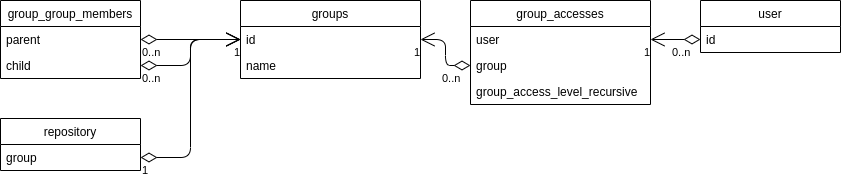
\includegraphics[width=\textwidth]{figures/group_system}
    \caption{Application groups system}
    \label{fig:group-system}
\end{figure}

This tree like groups' hierarchy allows us to easily give and take user access to any group.
If we want to change access from only parent group to also all subgroups access, we can simply toggle access{\_}level{\_}recursive
variable.
If we remove one particular group access, all other accesses remain in place, meaning that you some group was accessible
also via some other group access, you still have the access.

\section{Security}\label{sec:scurity}
Our application holds data, that shall not be visible to all client and therefore some kind of authentication and authorization methods are required.
For the data stored in Git notes we decided no extra security is required, as the time data isn't more sensitive than the actual code.
The security of source code stored in git repository is handled by a client himself and Git providers.
If they wish to have some more protection for git notes, they can configure it themselves.
We only provide the option to have notes only stored locally (not pushed to origin).

For the web application we need to implement our own security measures.
For most basic usage we have simple username and password authentication.
Accounts that only have password authentication are not authorized to access any groups nor repositories unless Admin user
explicitly gives them access to any.

To automatically get access to repositories you are contributor of you need to authenticate yourself via OAuth2 standard.
This way we can verify, that the user signing in to our application is the same user that has access to some git repository.

\subsection{OAuth2}\label{subsec:oauth2}
For OAuth2 authorization rocket{\_}oauth2 library is used, that follows RFC-6749 standard~\cite{rocket-oauth2, oauth2}.
We support authentication via Github.com, Gitlab.com, Bitbucket.org, Azure (Microsoft account) and TalTech gitlab server. % TODO: Add urls
First three were chosen as they are the most common git server providers as of 2021.
Authentication via Microsoft was added as TalTech (and also numerous other universities / companies) use it and therefore
all students have already registered account there.
Also, it provides access to user emails, that can be later used to filter out user commits.
TalTech gitlab server was added, as the application is currently developed for TalTech and therefore it was a requirement
that everything shall also work on TalTech gitlab server.

From all OAuth2 providers at least user read access is required to get access to user emails.
For OAuth2 providers, that are also a Git server providers also permissions to read user repositories data is required.
User repositories data is used to give user automatically access to his own repositories and also display repositories
not currently tracked by gtm.
It also allows more easily adding automatic data collection to user repositories, as user can browse through
repositories from different git server providers.

\subsection{Adding tracking to repositories}\label{subsec:adding-tracking}
We have added three levels to view time data:
\begin{enumerate}
    \item Add tracking (locally), view data via gtm CLI app.
    \item Add tracking (locally), log data to commit messages.
    \item Add tracking, sync data to gtm Web App.
\end{enumerate}

All smaller level can be included while using higher level option.  % TODO: koodi terminid spets fonti vms
Viewing data via CLI app is always possible, as it is the same app that is responsible for recording data.
This can be done both only locally or with pushing and pulling notes from remotes.
You can also add logging time spent to commit messages in both of the scenarios as it simply works on top of the already
existing system and only modifies commit message.
To use auto logging option you simply need to add --auto-log=[gitlab|jira] option when initiating tracking for a repository.

To view data from web interface, some more steps are required.
User flow for making repository visible on gtm web application is shown on Figure~\ref{fig:add-tracking-user-flow}.

\begin{figure}[h]
    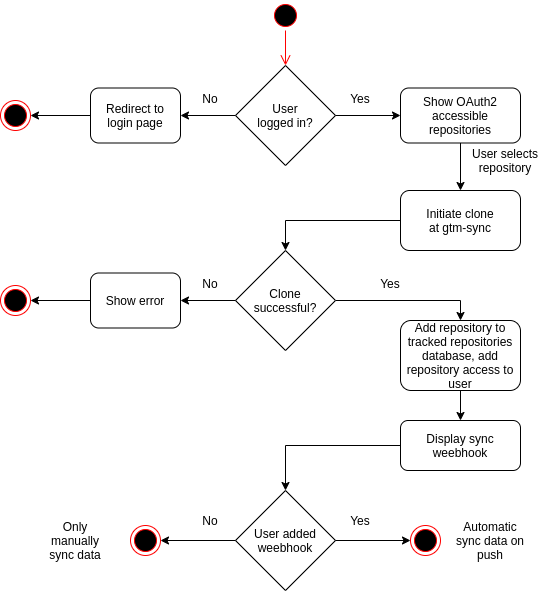
\includegraphics[width=\textwidth]{figures/add_repo_user_flow}
    \caption{Add tracking user flow}
    \label{fig:add-tracking-user-flow}
\end{figure}

Firstly, to have our sync client access the data, you cannot have time data only stored locally.
Then to add a repository, you need to have linked appropriate git server provider account via OAuth so that we can
verify that you have the access to repository.
After that you need to search for the repository from web interface and click add tracking button.
With that the tracking is technically added, but to also automatically sync time data on every push to remote,
you also need to add webhook.


\section{Backend}\label{sec:backend-content}
backend

\section{Frontend}\label{sec:frontend-content}
Frontend is one-page web application.
Users can log in and see their data according to their privileges.
This application has two main parts - profile and data visualization.
Under profile users can change password, link OAuth accounts and delete account.
Data visualization is divided into 3 parts - dashboard, leaderboard and timeline comparison.
In those tabs users can see their/others data as graphs and tables.

\subsection{Authentication and authorization}\label{subsec:authentication-and-authorization}
Authentication and authorization is implemented using bearer token system.
User gets token from api and stores it to the localstorage and adds to every request header.
User has to log in from log in page.
On success client receives json web token from backend and client stores it in localstorage.
Then user is automatically redirected to main page.
Users can log in with OAuth or username/password.
In case of OAuth user is redirected to according OAuth platform for authentication.
When successful, user is redirected to frontend with json web token.
Json web token is saved on localstorage and user is redirected to main page where he/she can access their data.
Login and register user flows are described on Figure
\ref{fig:login-signup-diagram}.

\begin{figure}[h]
    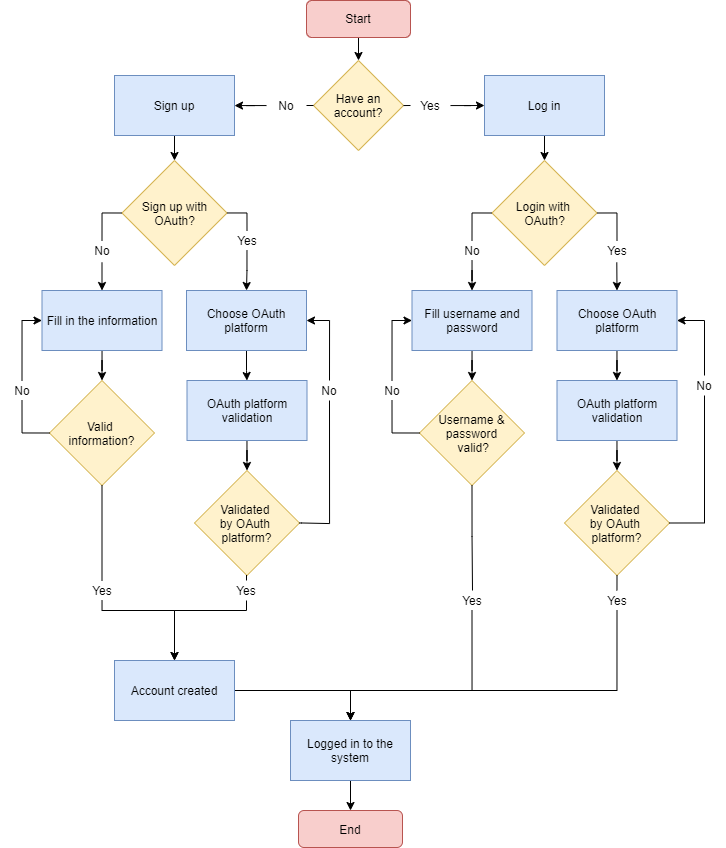
\includegraphics[width=\textwidth]{figures/login_signup_diagram}
    \caption{Log in and sign up flows}
    \label{fig:login-signup-diagram}
\end{figure}

\subsection{Profile}\label{subsec:profile}
\subsubsection{OAuth linking}\label{subsubsec:oauth-linking}
It is also possible to link multiple OAuth platforms to one account.
In that case user has to log in and head to the profile page where he/she can find link accounts tab.
If OAuth platform is already linked then backend unlinks it from this account, otherwise user is redirected to OAuth platform for authentication.
On success user will be redirected to frontend and user can access new repositories that this OAuth platform account has.
OAuth linking flow is described on Figure
\ref{fig:account-linking}.

\begin{figure}[h]
    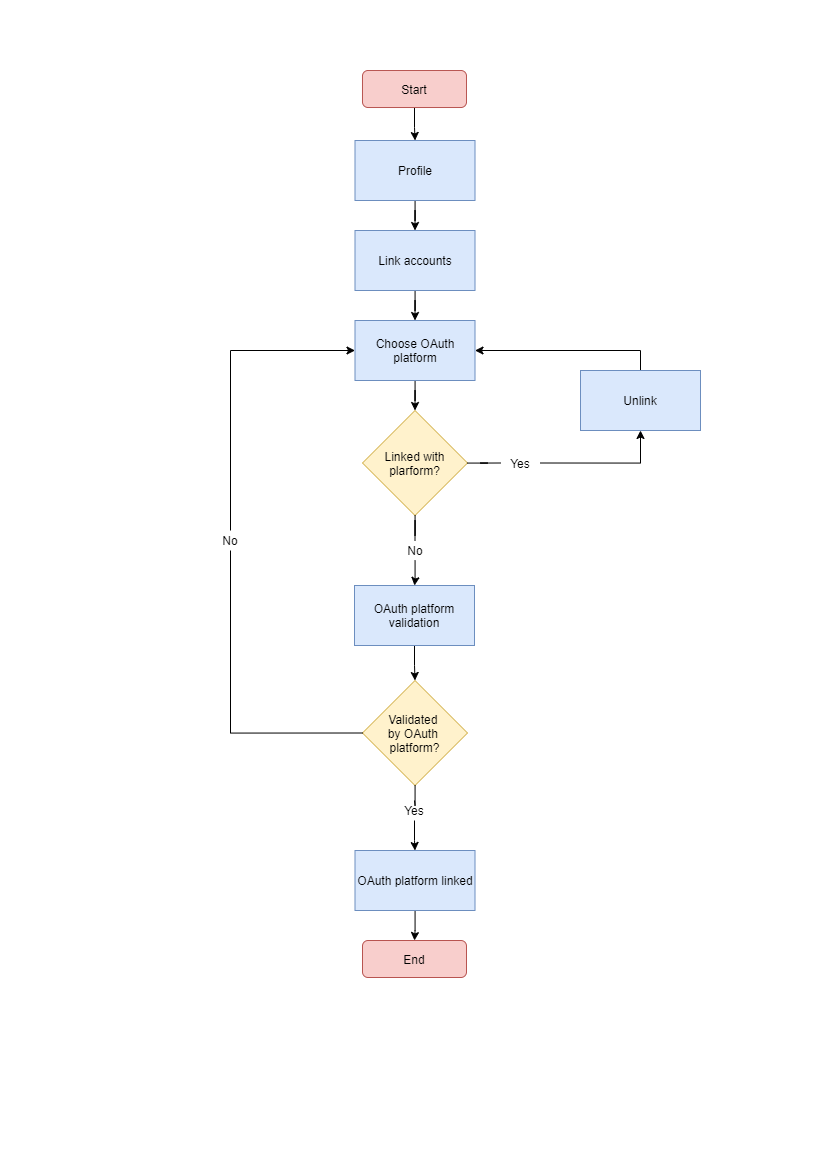
\includegraphics[width=\textwidth]{figures/account_linking.png}
    \caption{OAuth linking with user}
    \label{fig:account-linking}
\end{figure}

\subsubsection{Change password}\label{subsubsec:change-password}
Users can also change password.
In profile view under change password tab user has to fill all the fields correctly and password will be changed.
If user does not have a password (OAuth registration), only new password fields have to be filled.

\subsubsection{Delete account}\label{subsubsec:delete-account}
Account deletion is under delete account tab.
To keep away accidental account deletion user has to write their name to the input box and then can submit.
If account is deleted, user is redirected to the login page.


\subsection{Data visualization}\label{subsec:data-visualization}
Data visualization

\subsection{State management}\label{subsec:state-management-content}
State management
